\documentclass{article}
\usepackage[utf8x]{inputenc}

\usepackage[usenames,dvipsnames]{xcolor}
% \AddToHook{shipout/before}{%
%   \ifodd\value{page}
%     \pagecolor{blue!10!white}% Odd page colour (light blue)
%   \else
%     \pagecolor{red!10!white}% Even page colour (light red)
%   \fi
% }


\usepackage{geometry}
\geometry{letterpaper, margin=1in}

\providecommand{\tightlist}{%
  \setlength{\itemsep}{0pt}\setlength{\parskip}{0pt}}

\usepackage{adjustbox}
\usepackage[hyphens]{url}
\usepackage{lineno,hyperref}
\modulolinenumbers[5]

%% APA style
\usepackage{graphicx}
\usepackage{caption}

\definecolor{almond}{rgb}{0.94, 0.87, 0.8}
\usepackage{pagecolor}
\usepackage{afterpage}

\colorlet{normalcolor}{gray!70!Bittersweet!30}

\begin{document}
\pagestyle{empty}
\thispagestyle{empty}
\pagecolor{normalcolor!70}


%%%%

\begin{figure}[p]
\begin{adjustbox}{minipage=[c]{\textwidth-10mm},margin= 5mm 5mm 5mm 5mm, frame=1pt, bgcolor=almond,env=center}%
\begin{center}
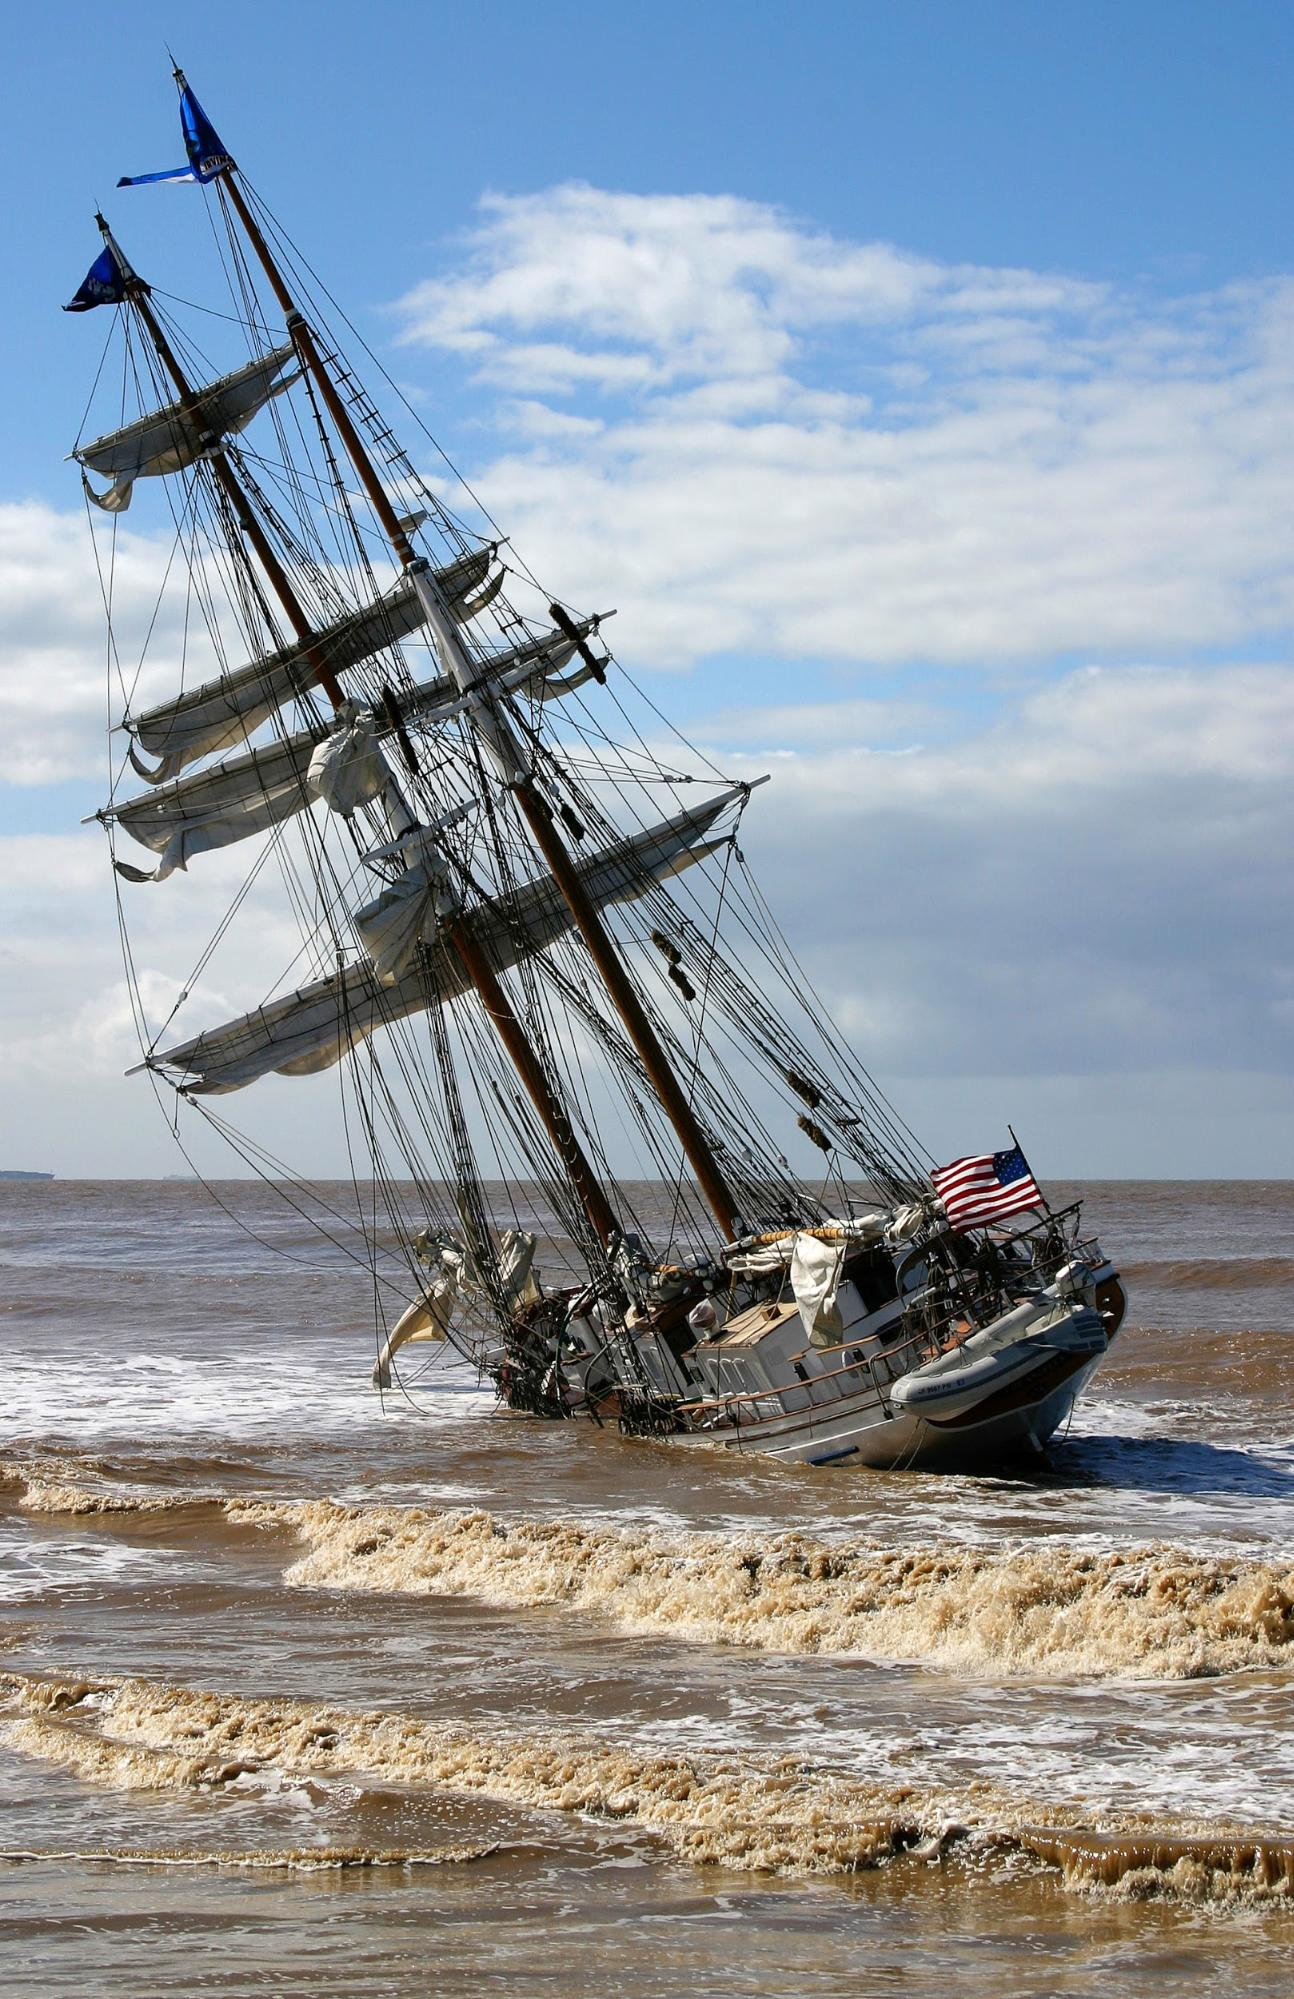
\includegraphics[width=.6\paperwidth,trim=0 6in 0 .7in,clip]{image3.jpg}
\end{center}

\begin{center}
\begin{minipage}[t]{0.7\paperwidth}\raggedright
\medskip
  
{\huge Participatory Scenario Planning}
\bigskip

\Large
\textbf{Context} you want to plan for possible future scenarios.\newline
\textbf{If} you have an interested group BUT no “expert” has all the answers;\newline
\textbf{Then} pool the collected expertise of the affected communities.\newline
% \textbf{Example} the Next Generation Services project (\url{http://nextgenpsf.co.uk}) used participatory scenario planning to imagine different plausible AI futures, which were then used in design sprints to expose professional services firms to potential AI challenges and opportunities.
\end{minipage}
\end{center}
\caption*{\emph{Image}:
The tall ship\href{https://en.wikipedia.org/wiki/Irving_Johnson_(ship)}{
}\href{https://en.wikipedia.org/wiki/Irving_Johnson_(ship)}{\emph{Irving
Johnson}} lies hard aground, only yards from shore, near the entrance to
Channel Islands
Harbor,\href{https://en.wikipedia.org/wiki/Oxnard,_California}{
}\href{https://en.wikipedia.org/wiki/Oxnard,_California}{\emph{Oxnard,
California}}, March 2005. US Coast Guard, public domain via Wikimedia commons.\newline 
\url{https://commons.wikimedia.org/wiki/File:IrvingJohnstonAground.jpg}}
\end{adjustbox}
\end{figure}

%%%

\begin{figure}[p]
\begin{adjustbox}{minipage=[c]{\textwidth-10mm},margin= 5mm 5mm 5mm 5mm, frame=1pt, bgcolor=almond,env=center}%
\begin{center}
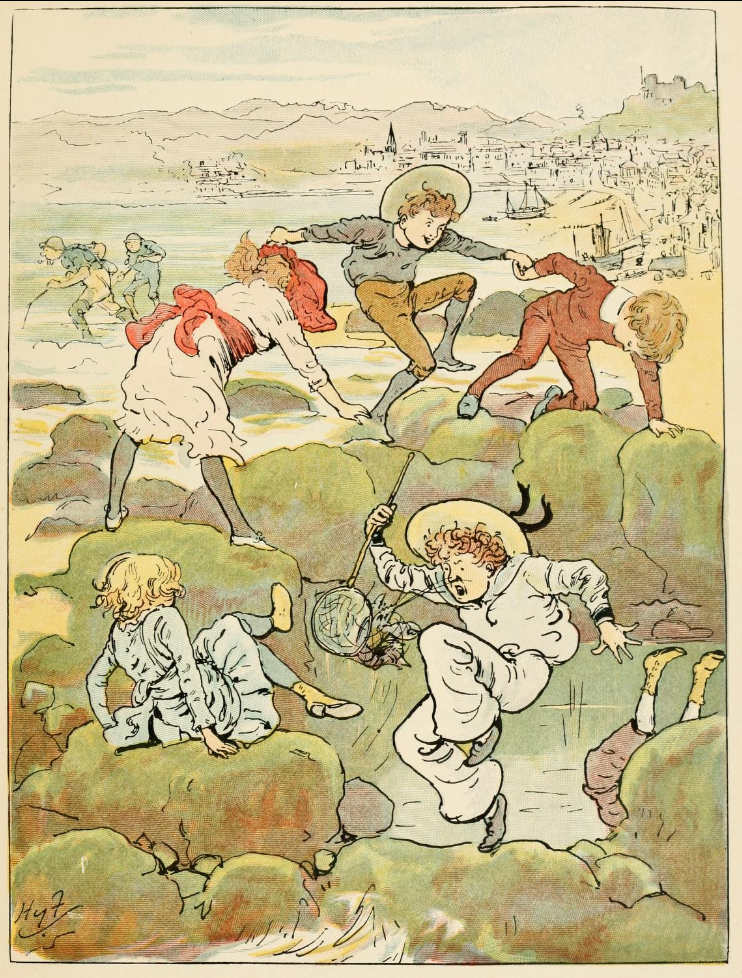
\includegraphics[width=.5\paperwidth]{image4.png}
\end{center}
\begin{center}
\begin{minipage}[t]{0.7\paperwidth}\raggedright
\medskip

{\huge Play to Anticipate the Future}
\bigskip

\Large
\textbf{Context} you want to have fun with friends, colleagues or acquaintances.\newline
\textbf{If} you want to explore possible futures BUT time travel does not exist and you don’t know what to expect;\newline
\textbf{Then} play a game that lets you experience a plausible future scenario together.\newline\smallskip

%\textbf{Example} a bipartisan group of politicians, former civilian and military officials, and academics gathered to play a scenario planning game to anticipate the possible aftermath of a contested election: at the very least the scenarios they came up with managed to surprise them (Bidgood, 2020).

\end{minipage}
\end{center}
\caption*{Image: illustration from
\href{https://archive.org/details/romps00furn/page/22/mode/2up}{\emph{Romps}}
by Harry Furniss, published by Routledge and Sons in 1886 (public domain
via Archive.org).\newline
\url{https://archive.org/details/romps00furn/page/22/mode/2up}}
\end{adjustbox}
\end{figure}

%%%

\begin{figure}[h]
\begin{adjustbox}{minipage=[c]{\textwidth-10mm},margin= 5mm 25mm 5mm 15mm, frame=1pt, bgcolor=almond,env=center}%
\begin{center}
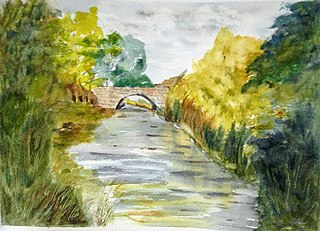
\includegraphics[width=.9\columnwidth]{image1.jpg}
\end{center}
\begin{center}
\begin{minipage}[t]{0.97\columnwidth}\raggedright
\medskip
{\huge Roadmap}
\bigskip

\Large
\textbf{Context} a group needs to coordinate its activities over a period of time.\newline
\textbf{If} the landscape is complex and not completely knowable BUT adjustment to action based on feedback is possible;\newline
\textbf{Then} use an explicit mechanism to share information about goals, obstacles, methods, and resources.\newline\smallskip
\bigskip

%\textbf{Example} Everyday roadmap languages include both iconic map and road sign symbols; when people are confused or lost they may ask for help or try to find their own way back to the road using other informal languages.

\end{minipage}
\end{center}
\vspace{1cm}
\caption*{Image: Maritess Sulcer, CC0, via Wikimedia
Commons\newline
\href{https://commons.wikimedia.org/wiki/File:Trees_and_bridge_and_stream_and_clouds_--_25_of_33.jpg}{\emph{https://commons.wikimedia.org/wiki/File:Trees\_and\_bridge\_and\_stream\_and\_clouds\_-\/-\_25\_of\_33.jpg}}}
\end{adjustbox}
\end{figure}

\end{document}